\documentclass{article}
\usepackage{tikz}
\usepackage[simplified]{pgf-umlcd}
\usepackage{multirow}
\usepackage{float}
\usetikzlibrary{arrows, arrows.meta}

\begin{document}

\title{
    Tarea 1 - Modelo y Diccionario \\
    INF239 - BASES DE DATOS
}
\author{
    Matias Peñaloza 202373037-8 \\
    Hans González 202373020-3
}
\date{
    2025-1
}
\maketitle

\section{Modelo}
\subsection{Entidad-Relación General}
Antes de realizar el modelo de la base de datos, analizaremos las entidades y relaciones presentes.

\begin{center}
\resizebox{0.8\textwidth}{!}{
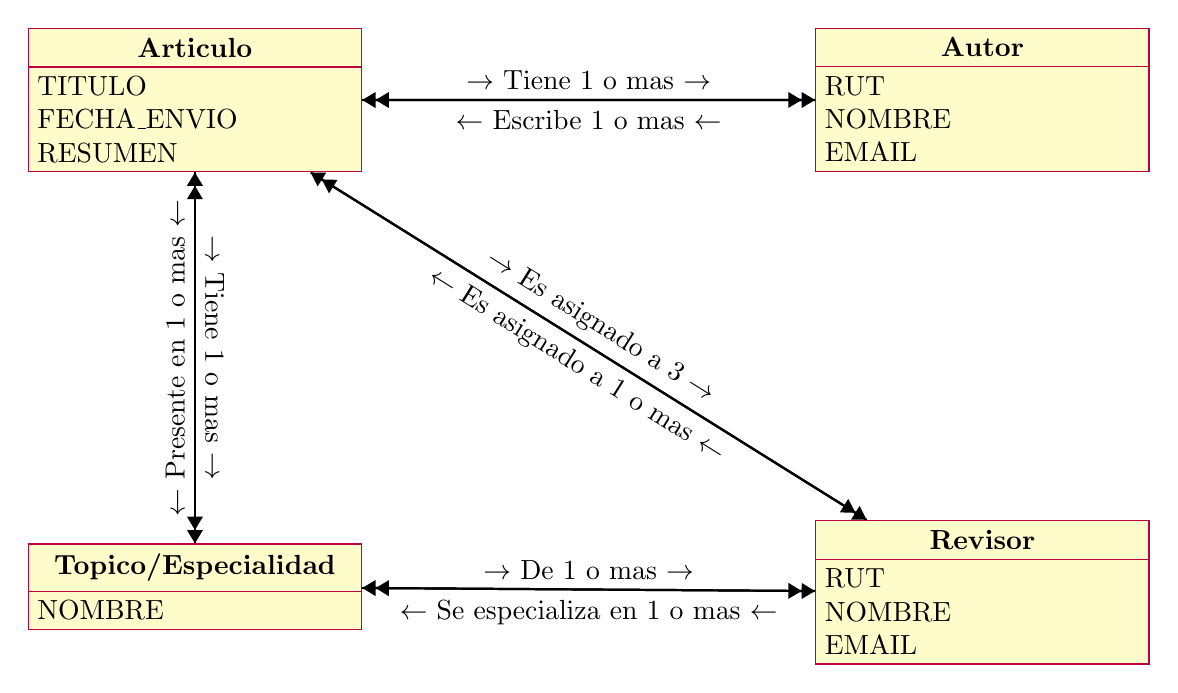
\begin{tikzpicture}
\begin{class}[text width=4cm]{Articulo}{0 ,0}
    \attribute{TITULO}
    \attribute{FECHA\_ENVIO}
    \attribute{RESUMEN}
\end{class}

\begin{class}[text width=4cm]{Autor}{10 ,0}
    \attribute{RUT}
    \attribute{NOMBRE}
    \attribute{EMAIL}
\end{class}

\begin{class}[text width=4cm]{Revisor}{10 ,-6.25}
    \attribute{RUT}
    \attribute{NOMBRE}
    \attribute{EMAIL}
\end{class}

\begin{class}[text width=4cm]{Topico/Especialidad}{0 ,-6.55}
    \attribute{NOMBRE}
\end{class}

\draw [thick,-{Triangle}{Triangle}] (Articulo) --++ (Revisor) node[midway, rotate=-32, above] {$\rightarrow$ Es asignado a 3 $\rightarrow$};
\draw [thick,-{Triangle}{Triangle}] (Revisor) --++ (Articulo) node[midway, rotate=-32, below] {$\leftarrow$ Es asignado a 1 o mas $\leftarrow$};

\draw [thick,-{Triangle}{Triangle}] (Articulo) --++ (Autor) node[midway, above] {$\rightarrow$ Tiene 1 o mas $\rightarrow$};
\draw [thick,-{Triangle}{Triangle}] (Autor) --++ (Articulo) node[midway, below] {$\leftarrow$ Escribe 1 o mas $\leftarrow$};

\draw [thick,-{Triangle}{Triangle}] (Revisor) --++ (Topico/Especialidad) node[midway, above] {$\rightarrow$ De 1 o mas $\rightarrow$};
\draw [thick,-{Triangle}{Triangle}] (Topico/Especialidad) --++ (Revisor) node[midway, below] {$\leftarrow$ Se especializa en 1 o mas $\leftarrow$};

\draw [thick,-{Triangle}{Triangle}] (Articulo) --++ (Topico/Especialidad) node[midway, rotate=-90, above] {$\rightarrow$ Tiene 1 o mas $\rightarrow$};
\draw [thick,-{Triangle}{Triangle}] (Topico/Especialidad) --++ (Articulo) node[midway, rotate=90, above] {$\leftarrow$ Presente en 1 o mas $\leftarrow$};

\end{tikzpicture}
}
\end{center}

\subsection{Modelo BD}
Ahora podemos llevar el modelo general de la situacion a un modelo de base de datos.

\begin{center}
\resizebox{0.8\textwidth}{!}{
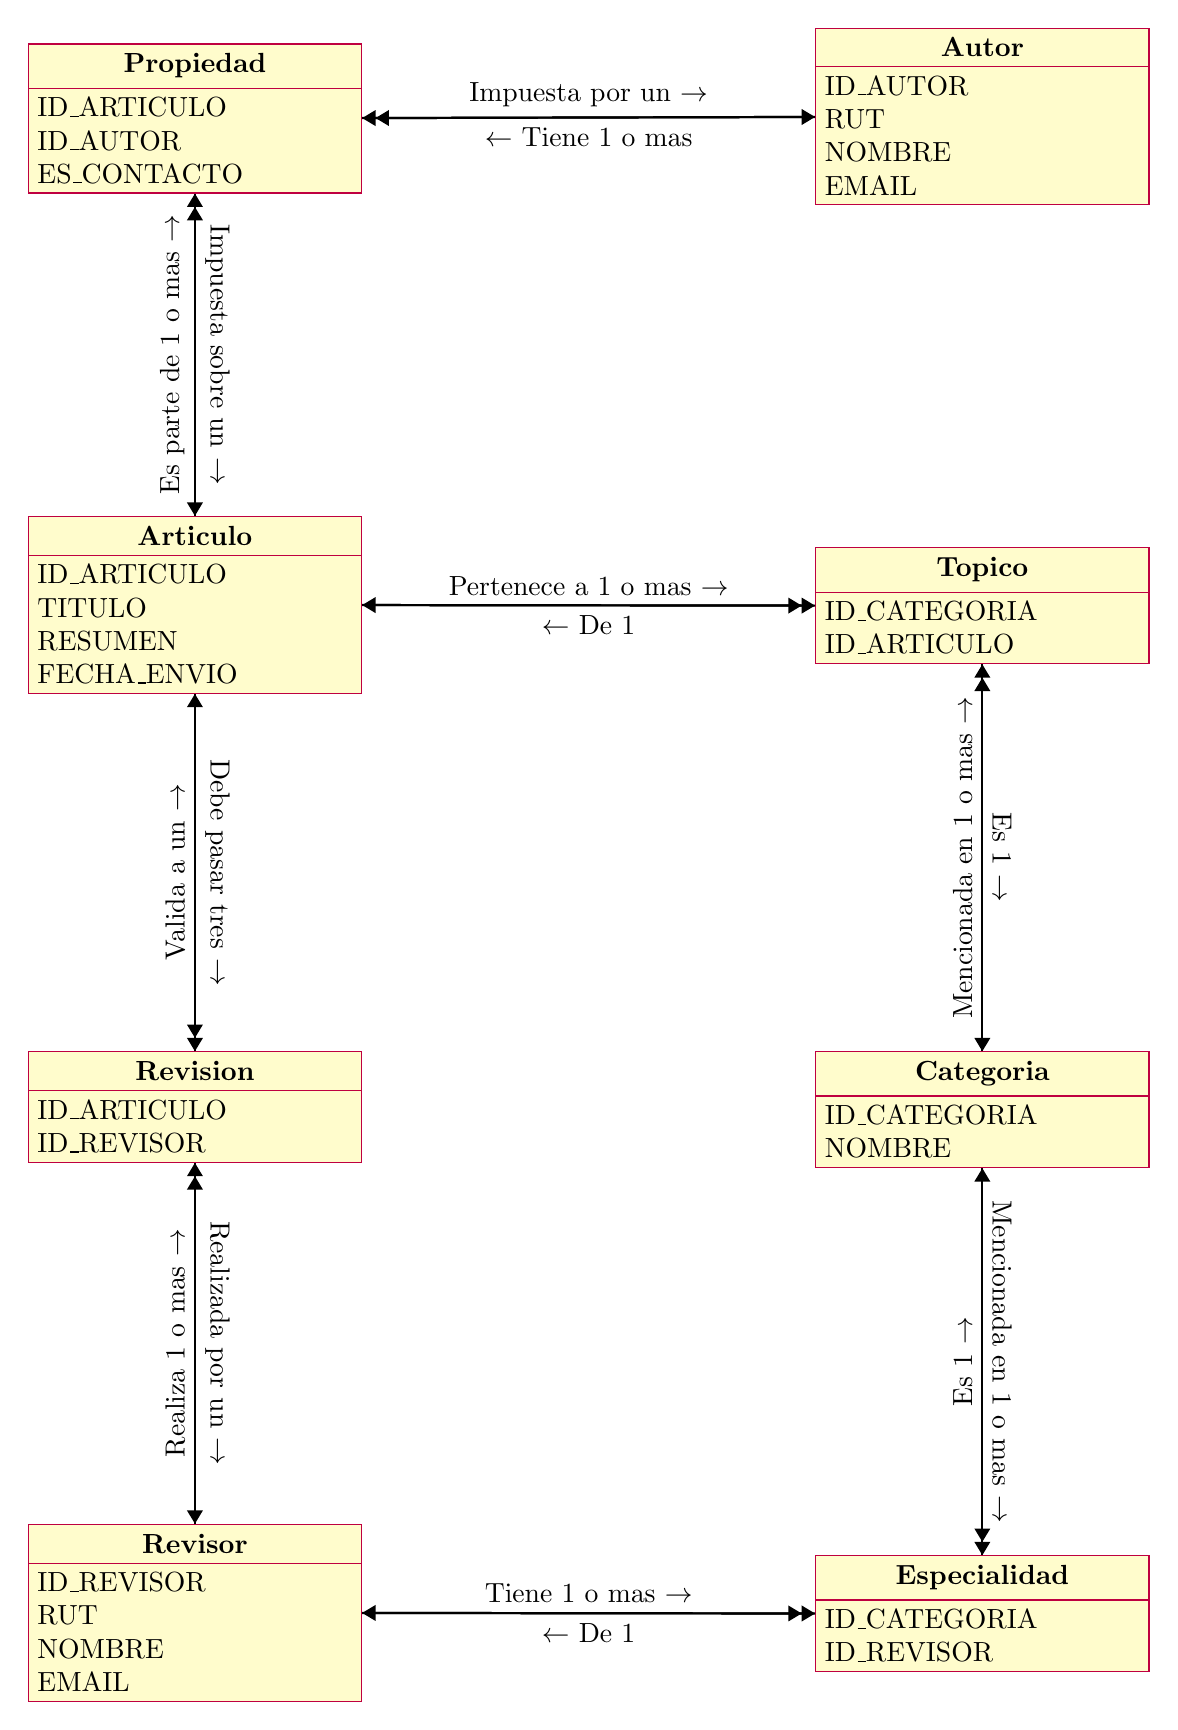
\begin{tikzpicture}
    \begin{class}[text width=4cm]{Articulo}{-1 ,-3.2}
        \attribute{ID\_ARTICULO}
        \attribute{TITULO}
        \attribute{RESUMEN}
        \attribute{FECHA\_ENVIO}
    \end{class}

    \begin{class}[text width=4cm]{Propiedad}{-1 ,2.8}
        \attribute{ID\_ARTICULO}
        \attribute{ID\_AUTOR}
        \attribute{ES\_CONTACTO}
    \end{class}

    \begin{class}[text width=4cm]{Autor}{9 ,3}
        \attribute{ID\_AUTOR}
        \attribute{RUT}
        \attribute{NOMBRE}
        \attribute{EMAIL}
    \end{class}

    \begin{class}[text width=4cm]{Revision}{-1 ,-10}
        \attribute{ID\_ARTICULO}
        \attribute{ID\_REVISOR}
    \end{class}

    \begin{class}[text width=4cm]{Revisor}{-1 ,-16}
        \attribute{ID\_REVISOR}
        \attribute{RUT}
        \attribute{NOMBRE}
        \attribute{EMAIL}
    \end{class}

    \begin{class}[text width=4cm]{Especialidad}{9 ,-16.4}
        \attribute{ID\_CATEGORIA}
        \attribute{ID\_REVISOR}
    \end{class}

    \begin{class}[text width=4cm]{Topico}{9 ,-3.6}
        \attribute{ID\_CATEGORIA}
        \attribute{ID\_ARTICULO}
    \end{class}

    \begin{class}[text width=4cm]{Categoria}{9 ,-10}
        \attribute{ID\_CATEGORIA}
        \attribute{NOMBRE}
    \end{class}

    \draw [thick,-{Triangle}{Triangle}] (Articulo) --++ (Revision) node[midway, rotate=90, above] {Valida a un $\rightarrow$};
    \draw [thick, -{Triangle}] (Revision) --++ (Articulo) node[midway, rotate=-90, above] {Debe pasar tres $\rightarrow$};

    \draw [thick,-{Triangle}{Triangle}] (Revisor) --++ (Revision) node[midway, rotate=-90, above] {Realizada por un $\rightarrow$};
    \draw [thick, -{Triangle}] (Revision) --++ (Revisor) node[midway, rotate=90, above] {Realiza 1 o mas $\rightarrow$};

    \draw [thick,-{Triangle}{Triangle}] (Articulo) --++ (Propiedad) node[midway, rotate=90, above] {Es parte de 1 o mas $\rightarrow$};
    \draw [thick, -{Triangle}] (Propiedad) --++ (Articulo) node[midway, rotate=-90, above] {Impuesta sobre un $\rightarrow$};

    \draw [thick,-{Triangle}{Triangle}] (Autor) --++ (Propiedad) node[midway, above] {Impuesta por un $\rightarrow$};
    \draw [thick, -{Triangle}] (Propiedad) --++ (Autor) node[midway, below] {$\leftarrow$ Tiene 1 o mas};

    \draw [thick,-{Triangle}{Triangle}] (Revisor) --++ (Especialidad) node[midway, above] {Tiene 1 o mas $\rightarrow$};
    \draw [thick, -{Triangle}] (Especialidad) --++ (Revisor) node[midway, below] {$\leftarrow$ De 1};

    \draw [thick,-{Triangle}{Triangle}] (Articulo) --++ (Topico) node[midway, above] {Pertenece a 1 o mas $\rightarrow$};
    \draw [thick, -{Triangle}] (Topico) --++ (Articulo) node[midway, below] {$\leftarrow$ De 1};

    \draw [thick,-{Triangle}{Triangle}] (Categoria) --++ (Topico) node[midway, rotate=90, above] {Mencionada en 1 o mas $\rightarrow$};
    \draw [thick, -{Triangle}] (Topico) --++ (Categoria) node[midway, rotate=-90, above] {Es 1 $\rightarrow$};

    \draw [thick,-{Triangle}{Triangle}] (Categoria) --++ (Especialidad) node[midway, rotate=-90, above] {Mencionada en 1 o mas $\rightarrow$};
    \draw [thick, -{Triangle}] (Especialidad) --++ (Categoria) node[midway, rotate=90, above] {Es 1 $\rightarrow$};

\end{tikzpicture}
}
\end{center}




\section{Diccionario de Datos}

\subsection{Tabla: Categoria}
\begin{table}[H]
\centering
\begin{tabular}{|l|l|l|l|p{6cm}|}
\hline
\textbf{Atributo} & \textbf{Tipo de Dato} & \textbf{Nullable} & \textbf{Unique} & \textbf{Descripción} \\ \hline
id\_categoria & SERIAL & NO & YES & Identificador único de la categoría. \\ \hline
nombre & VARCHAR(85) & NO & NO & Nombre de la categoría. \\ \hline
\end{tabular}
\caption{Diccionario de datos de la tabla Categoria}
\label{tab:categoria}
\end{table}

\subsection{Tabla: Articulo}
\begin{table}[H]
\centering
\begin{tabular}{|l|l|l|l|p{6cm}|}
\hline
\textbf{Atributo} & \textbf{Tipo de Dato} & \textbf{Nullable} & \textbf{Unique} & \textbf{Descripción} \\ \hline
id\_articulo & SERIAL & NO & YES & Identificador único del artículo. \\ \hline
titulo & VARCHAR(50) & NO & NO & Título del artículo. \\ \hline
resumen & VARCHAR(150) & NO & NO & Resumen del contenido del artículo. \\ \hline
fecha\_envio & DATE & NO & NO & Fecha en que se envió el artículo. \\ \hline
\end{tabular}
\caption{Diccionario de datos de la tabla Articulo}
\label{tab:articulo}
\end{table}

\subsection{Tabla: Topico}
\begin{table}[H]
\centering
\begin{tabular}{|l|l|l|l|p{6cm}|}
\hline
\textbf{Atributo} & \textbf{Tipo de Dato} & \textbf{Nullable} & \textbf{Unique} & \textbf{Descripción} \\ \hline
id\_categoria & INTEGER & NO & NO & Identificador de la categoría asociada. \\ \hline
id\_articulo & INTEGER & NO & NO & Identificador del artículo asociado. \\ \hline
\end{tabular}
\caption{Diccionario de datos de la tabla Topico}
\label{tab:topico}
\end{table}

\subsection{Tabla: Autor}
\begin{table}[H]
\centering
\begin{tabular}{|l|l|l|l|p{6cm}|}
\hline
\textbf{Atributo} & \textbf{Tipo de Dato} & \textbf{Nullable} & \textbf{Unique} & \textbf{Descripción} \\ \hline
id\_autor & SERIAL & NO & YES & Identificador único del autor. \\ \hline
rut & CHAR(10) & NO & YES & RUT único del autor. \\ \hline
nombre & VARCHAR(85) & NO & NO & Nombre completo del autor. \\ \hline
email & VARCHAR(95) & NO & YES & Correo electrónico único del autor. \\ \hline
\end{tabular}
\caption{Diccionario de datos de la tabla Autor}
\label{tab:autor}
\end{table}

\subsection{Tabla: Propiedad}
\begin{table}[H]
\centering
\begin{tabular}{|l|l|l|l|p{6cm}|}
\hline
\textbf{Atributo} & \textbf{Tipo de Dato} & \textbf{Nullable} & \textbf{Unique} & \textbf{Descripción} \\ \hline
id\_articulo & INTEGER & NO & NO & Identificador del artículo asociado. \\ \hline
id\_autor & INTEGER & NO & NO & Identificador del autor asociado. \\ \hline
es\_contacto & BOOLEAN & NO & NO & Indica si el autor es el contacto principal. \\ \hline
\end{tabular}
\caption{Diccionario de datos de la tabla Propiedad}
\label{tab:propiedad}
\end{table}

\subsection{Tabla: Revisor}
\begin{table}[H]
\centering
\begin{tabular}{|l|l|l|l|p{6cm}|}
\hline
\textbf{Atributo} & \textbf{Tipo de Dato} & \textbf{Nullable} & \textbf{Unique} & \textbf{Descripción} \\ \hline
id\_revisor & SERIAL & NO & YES & Identificador único del revisor. \\ \hline
rut & CHAR(10) & NO & YES & RUT único del revisor. \\ \hline
nombre & VARCHAR(85) & NO & NO & Nombre completo del revisor. \\ \hline
email & VARCHAR(95) & NO & YES & Correo electrónico único del revisor. \\ \hline
\end{tabular}
\caption{Diccionario de datos de la tabla Revisor}
\label{tab:revisor}
\end{table}

\subsection{Tabla: Especialidad}
\begin{table}[H]
\centering
\begin{tabular}{|l|l|l|l|p{6cm}|}
\hline
\textbf{Atributo} & \textbf{Tipo de Dato} & \textbf{Nullable} & \textbf{Unique} & \textbf{Descripción} \\ \hline
id\_categoria & INTEGER & NO & NO & Identificador de la categoría asociada. \\ \hline
id\_revisor & INTEGER & NO & NO & Identificador del revisor asociado. \\ \hline
\end{tabular}
\caption{Diccionario de datos de la tabla Especialidad}
\label{tab:especialidad}
\end{table}

\subsection{Tabla: Revision}
\begin{table}[H]
\centering
\begin{tabular}{|l|l|l|l|p{6cm}|}
\hline
\textbf{Atributo} & \textbf{Tipo de Dato} & \textbf{Nullable} & \textbf{Unique} & \textbf{Descripción} \\ \hline
id\_articulo & INTEGER & NO & NO & Identificador del artículo revisado. \\ \hline
id\_revisor & INTEGER & NO & NO & Identificador del revisor asociado. \\ \hline
\end{tabular}
\caption{Diccionario de datos de la tabla Revision}
\label{tab:revision}
\end{table}

\end{document}
